%% arara directives
% arara: xelatex
% arara: bibtex
% arara: xelatex
% arara: xelatex

%\documentclass{article} % One-column default
\RequirePackage[2020-02-02]{latexrelease}
\documentclass[twocolumn, switch]{article} % Method A for two-column formatting

\usepackage{preprint}

%% Math packages
\usepackage{amsmath, amsthm, amssymb, amsfonts}

%% Bibliography options
\usepackage[numbers,square]{natbib}
\bibliographystyle{unsrtnat}
%\usepackage{natbib}
%\bibliographystyle{Geology}

%% General packages
\usepackage[utf8]{inputenc}	% allow utf-8 input
\usepackage[T1]{fontenc}	% use 8-bit T1 fonts
\usepackage{xcolor}		% colors for hyperlinks
\usepackage{graphicx}
\graphicspath{{./assets/}}
\usepackage[colorlinks = true,
            linkcolor = purple,
            urlcolor  = blue,
            citecolor = cyan,
            anchorcolor = black]{hyperref}	% Color links to references, figures, etc.
\usepackage{booktabs} 		% professional-quality tables
\usepackage{nicefrac}		% compact symbols for 1/2, etc.
\usepackage{microtype}		% microtypography
\usepackage{lineno}		% Line numbers
\usepackage{float}			% Allows for figures within multicol
%\usepackage{multicol}		% Multiple columns (Method B)

\usepackage{lipsum}		%  Filler text

 %% Special figure caption options
\usepackage{newfloat}
\DeclareFloatingEnvironment[name={Supplementary Figure}]{suppfigure}
\usepackage{sidecap}
\sidecaptionvpos{figure}{c}

% Section title spacing  options
\usepackage{titlesec}
\titlespacing\section{0pt}{12pt plus 3pt minus 3pt}{1pt plus 1pt minus 1pt}
\titlespacing\subsection{0pt}{10pt plus 3pt minus 3pt}{1pt plus 1pt minus 1pt}
\titlespacing\subsubsection{0pt}{8pt plus 3pt minus 3pt}{1pt plus 1pt minus 1pt}

% ORCiD insertion
\usepackage{tikz,xcolor,hyperref}

\definecolor{lime}{HTML}{A6CE39}
\DeclareRobustCommand{\orcidicon}{
	\begin{tikzpicture}
	\draw[lime, fill=lime] (0,0) 
	circle [radius=0.16] 
	node[white] {{\fontfamily{qag}\selectfont \tiny ID}};
	\draw[white, fill=white] (-0.0625,0.095) 
	circle [radius=0.007];
	\end{tikzpicture}
	\hspace{-2mm}
}
\foreach \x in {A, ..., Z}{\expandafter\xdef\csname orcid\x\endcsname{\noexpand\href{https://orcid.org/\csname orcidauthor\x\endcsname}
			{\noexpand\orcidicon}}
}
% Define the ORCID iD command for each author separately. Here done for two authors.
\newcommand{\orcidauthorA}{0000-0000-0000-0001}
\newcommand{\orcidauthorB}{0000-0000-0000-0002}
\newcommand{\orcidauthorC}{0000-0000-0000-0003}
\newcommand{\orcidauthorD}{0000-0000-0000-0004}

%%%%%%%%%%%%%%%%   Title   %%%%%%%%%%%%%%%%
\title{Machine Learning techniques for malicious PDF detection}

% Add watermark with submission status
\usepackage{xwatermark}
% Left watermark
\newwatermark[firstpage,color=gray!60,angle=90,scale=0.32, xpos=-4.05in,ypos=0]{\href{https://doi.org/}{\color{gray}{Publication doi}}}
% Right watermark
\newwatermark[firstpage,color=gray!60,angle=90,scale=0.32, xpos=3.9in,ypos=0]{\href{https://doi.org/}{\color{gray}{Preprint doi}}}
% Bottom watermark
\newwatermark[firstpage,color=gray!90,angle=0,scale=0.28, xpos=0in,ypos=-5in]{*correspondence: \texttt{email@institution.edu}}
%%%%%%%%%%%%%%%  AUTHORS LIST  %%%%%%%%%%%%%%%
\usepackage{authblk}
\renewcommand*{\Authfont}{\bfseries}
\author{Lorenzo Ippolito, Mattia Rosso, Martino Picasso}


%%%%%%%%%%%%%%    Front matter    %%%%%%%%%%%%%%
\begin{document}

\twocolumn[ % Method A for two-column formatting
	\begin{@twocolumnfalse} % Method A for two-column formatting

		\maketitle
		%%%# ABSTRACT #%%
		\begin{abstract}
			This project presents a thorough analysis of machine learning techniques for detecting malicious PDF files. By comparing the performance of three binary classification models - K-Nearest Neighbors (KNN), Support Vector Machines (SVM), and Decision Trees - we demonstrate the effectiveness of these approaches in achieving high accuracy and low false negative rates.
			What makes this project stand out is its focus on the machine learning models themselves, including the careful selection of hyperparameters to optimize their performance. Additionally, the inclusion of KNN as a valid model is rare in the field, and the analysis of evasion techniques adds another layer of depth to the study. Overall, this paper offers a comprehensive look at the use of machine learning for malicious PDF detection and the potential vulnerabilities of these models.
		\end{abstract}
		%\keywords{First keyword \and Second keyword \and More} % (optional)
		\vspace{0.35cm}

	\end{@twocolumnfalse} % Method A for two-column formatting
] % Method A for two-column formatting

%\begin{multicols}{2} % Method B for two-column formatting (doesn't play well with line numbers), comment out if using method A


%%%%%%%%%%%%%%%  Main text   %%%%%%%%%%%%%%%
% \linenumbers

%%%# INTRODUCTION #%%
\section{Introduction}
PDF (Portable Document Format) is a widely used file format for exchanging and sharing documents. It is a versatile format that can contain a variety of different types of content, including text, images, multimedia, and executable code. In this section, we will examine the structure of PDF files and the various elements that can be used to specify the contents of a PDF.
One important aspect of PDF structure is the use of keywords, also known as actions or triggers. These keywords are used to specify different types of content, such as JavaScript code, images, and multimedia. In our analysis of malicious PDF files, we have focused on a set of keywords that are commonly known to be discriminant for static PDF malware analysis. By examining the presence of these keywords in a PDF, we can characterize the file and determine whether it may be malicious.
In addition to keywords, PDF files can also contain other types of elements, such as fonts, annotations, and form fields. These elements can be used to specify the appearance and interactive features of a PDF, but they can also be exploited for malicious purposes. For example, a PDF may contain a hidden form field that is used to exfiltrate sensitive information from the victim's computer.
In summary, the structure of a PDF file is an important factor to consider when detecting malicious content. By analyzing the keywords and other elements present in a PDF, we can gain insight into its contents and determine whether it may be malicious.

History of PDF attacks
The flexibility and widespread adoption of PDF also make it a popular choice for delivering malicious content. In this chapter, we will review the history of PDF attacks and the various types of malicious content that have been delivered via PDF files.
The first known PDF attack occurred in 2005, when a malicious PDF file was used to deliver the Trojan horse malware known as "Zotob." This malware exploited a vulnerability in Microsoft Windows and was used to take control of infected computers. Since then, PDF files have been used to deliver a wide range of malware, including ransomware, spyware, and adware.
In addition to malware, PDF files have also been used to deliver phishing attacks and other forms of cyber threats. For example, a PDF file may contain a link to a fake login page or a form that asks the user to enter sensitive information, such as passwords or credit card numbers. By tricking the user into entering this information, the attacker can gain access to their accounts or steal their identity.
Another common type of PDF attack is the use of "exploit kits." These kits are collections of tools that can be used to exploit vulnerabilities in software and deliver malware via PDF files. One well-known exploit kit is "Blackhole," which was used to deliver a variety of malware, including the "Citadel" banking Trojan.


%%# RELATED WORK #%%
\section{Related work}
\label{sec:relatedwork}
See Section \ref{sec:relatedwork}.
\subsection{Related work: second level}
\subsubsection{Related work: third level}
\paragraph{Paragraph}
\cite{kour2014real,kour2014fast}
\cite{hadash2018estimate}.
\begin{quote}
	Hasselmo, et al.\ (1995) investigated\dots
\end{quote}

\begin{figure}[H]
	\centering
	\fbox{\rule[-.5cm]{4cm}{4cm} \rule[-.5cm]{4cm}{0cm}}
	\caption{Sample figure caption.}
	\label{fig:fig1}
\end{figure}
\begin{itemize}
	\item a
	\item b
	\item c
\end{itemize}

%%# DATASETS AND FEATURES #%%
\section{Datasets and features}
\label{sec:datasetsandfeatures}
In this chapter, we will discuss the data sources and extraction process for our machine learning model for detecting malicious PDFs.
As the first step in building our model, we needed to obtain a dataset of PDFs to use for training and evaluation. After reviewing several options, we decided to use the Contagio dataset for our work. The Contagio dataset is a collection of malicious PDF files that has been widely used for research and testing purposes. The dataset was created by the security firm Mandiant and contains about 20000 PDF samples, including malware, phishing attacks, and other types of malicious content. The samples in the dataset are organized into various categories, such as exploit kits, banking Trojans, and ransomware, and are representative of the types of threats that are commonly encountered in the wild. This dataset has been cited in many publications on the topic of malicious PDF detection, and it provides a balanced number of both malicious and benign PDFs. By using this dataset, we can compare our results to those reported in previous publications and see if our models are performing better or worse.
Next, we needed to extract the data from the PDFs in order to use it for training and evaluation. We chose to perform a static analysis, which does not require opening the PDFs in a reader. Instead, we used a tool called PDFId to extract relevant information from the PDFs. PDFId characterizes each PDF by extracting the number of occurrences of specific keywords. This allows us to map each PDF into an array of 22 elements, with each element representing the count of a specific keyword. We are therefore working with samples of 22 integer features.
We report here the features used with a short summary of their meaning and use:
\begin{itemize}
	\item obj: It is used to specify the start of an object in a PDF file. An object can be a variety of types of data, such as text, images, or executable code.
	\item endobj: It is used to specify the end of an object in a PDF file. It marks the end of the data associated with a particular object.
	\item stream: It is used to specify the start of a stream of data in a PDF file. A stream is a contiguous sequence of data that is usually compressed and can be a variety of types, such as text, images, or audio.
	\item endstream: It is used to specify the end of a stream of data in a PDF file. It marks the end of the data associated with a particular stream.
	\item xref: It is used to specify a cross-reference table in a PDF file. The cross-reference table contains information about the objects in the PDF file, including their location and size.
	\item trailer: It is used to specify the trailer of a PDF file. The trailer contains information about the structure of the PDF file, such as the location of the cross-reference table and the root object.
	\item startxref: It is used to specify the starting position of the cross-reference table in a PDF file. It is typically located at the end of the file and is used to locate the objects in the PDF file.
	\item /Page: It is used to specify a page object in a PDF file. A page object represents a single page in the PDF document and contains information about the layout and content of the page.
	\item /Encrypt: It is used to specify that a PDF file is encrypted. Encrypted PDF files are protected with a password and cannot be viewed or edited without the correct password.
	\item /ObjStm: It is used to specify an object stream in a PDF file. An object stream is a stream of data that contains multiple objects, which are compressed and stored in a single stream to save space.
	\item /JS: It is used to specify that a PDF file contains JavaScript code. JavaScript is a programming language that can be used to create interactive features in a PDF file, but it can also be used for malicious purposes.
	\item /JavaScript: It is similar to the /JS keyword and is used to specify that a PDF file contains JavaScript code.
	\item /AA: It is used to specify that a PDF file contains additional actions. Additional actions are additional instructions or triggers that are executed when certain events occur, such as when the PDF file is opened or a form is submitted.
	\item /OpenAction: It is used to specify an action that is executed when a PDF file is opened. This action can be used to execute code or perform other tasks.
	\item /AcroForm: It is used to specify that a PDF file contains interactive form fields. Form fields can be used to create interactive forms that can be filled out by the user, but they can also be used for malicious purposes, such as exfiltrating sensitive information from the user.
	\item /JBIG2Decode: It is used to specify that a PDF file contains JBIG2 encoded data. JBIG2 is a compression algorithm that is used to compress black and white images, and is often used in PDF files to reduce the size of scanned documents.
	\item /RichMedia: It is used to specify that a PDF file contains rich media content, such as audio or video. Rich media can be used to enhance the interactive experience of a PDF file, but it can also be used to deliver malware or other malicious content.
	\item /Launch: It is used to specify an action that is executed when a PDF file is opened. This action can be used to launch a program or open a file, and is often used to deliver malware or other malicious content.
	\item /EmbeddedFile: It is used to specify that a PDF file contains an embedded file. An embedded file is a file that is stored within the PDF file and can be extracted and accessed by the user.
	\item /XFA: It is used to specify that a PDF file contains an XFA (XML Forms Architecture) form. XFA forms are used to create interactive forms that can be filled out by the user, and are often used in conjunction with AcroForms.
	\item /Colors: It is used to specify that a PDF file contains more than 16 million colors. This is typically an indication of high-quality images or graphics, but it can also be used to identify malicious PDF files that use large images or graphics to hide their contents.
\end{itemize}

The output of PDFId is then converted into a CSV file, which can be easily accessed using the numpy and pandas libraries. This CSV file serves as the basis for our data extraction pipeline, which we have implemented using the functions provided by PDFId. It is important to note that PDFId is a tool specifically designed for the analysis of malicious PDFs, as the 22 keywords it extracts are well known to be discriminant for PDF malware analysis. These keywords do not represent the full set of possible keywords that may appear in a PDF file.
For our classification task, we will be performing a binary classification, with malicious PDFs being labelled as positive samples and benign PDFs being labelled as negative samples. This allows us to easily train and evaluate our models, as we only need to predict whether a given PDF is malicious or not.

\subsubsection{Model validation}
In this chapter, we will discuss the methods we used to validate the models developed in our study of machine learning techniques for malicious PDF detection. Model validation is an important step in the development of any machine learning model, as it allows us to assess the performance of the model and identify any issues or biases that may affect its accuracy.
One method we used for model validation was a static train-test split. In this approach, we split all of the samples in our dataset into two sets: a training set and a test set. The training set, which consists of 80\% of the samples, is used to train and validate the models using a k-fold cross validation approach. The test set, which consists of 20\% of the samples, is not used to make decisions during the model building phase, but is instead used to make final considerations about the performance of the models trained with the best parameters/hyperparameters.
To evaluate the performance of our models, we used two measures: the False Negative Rate (FNR) and Accuracy. The FNR is defined as
\begin{center}
	$FNR = \frac{FN}{FN + TP}$
\end{center}
We aimed to minimize the FNR as much as possible, as False Negatives can be particularly damaging in the context of malicious PDF detection. False Negatives can lead to the failure to detect and prevent attacks and can have serious consequences for individuals and organizations.
At the same time, we also took into consideration the value of Accuracy, as the penalization of False Negative errors should not result in an excessively high number of False Positive errors. It is important to find a balance between minimizing False Negatives and minimizing False Positives, as both can have negative consequences. False Positives can lead to unnecessary alerts and can waste resources and can also erode trust in the system.
In addition to the static train-test split and the measures of FNR and Accuracy, we also used other techniques to validate our models. For example, we used cross-validation to ensure that our models were not overfitting to the training data and to identify the optimal hyperparameters for each model.

%%# SVM #%%
\section{Support vector machines}
\label{sec:svm}
% Intro that motivates why we use SVM (citing papers of \ref{sec:relatedwork})
Support Vector Machines are linear classifiers that look for maximum margin separation hyperplanes. The primal formulation of the soft-margin SVM problem consists in minimizing the function:
\begin{center}
	$J(w,w_0) = \frac{1}{2}||w||^2 + C\sum_{i=1}^{n}\xi_i$ \\
	s.t. $z_i(w^Tx_i+w_0) \ge 1 - \xi_i$ \\
	and $\xi_i \ge 0$
\end{center}
To define the hard margin SVM problem the penalty term $C\sum_{i=1}^{n}\xi_i$ has been added to the soft margin SVM problem. $\xi_i$ are slack variables and estimate the number of missclassified samples. The hyperparameter C is meant to define the strongness of this penalization. We also introduce the dual problem that, besides the fact that is the one that $sklearn$ optimizes, is also useful to explain how the adversarial samples will be crafted in section \ref
{sec:attacks}.
\begin{center}
	\label{dualproblem}
	$J_D(\alpha) = \sum_{i=1}^{n}\alpha_i -\frac{1}{2}\sum_{i=1}^{n}\sum_{j=1}^{n}\alpha_i\alpha_jz_iz_jx_{i}^Tx_j$\\
	s.t. $0 \le \alpha_i \le C$ \\
	and $\sum_{i=1}^{n}\alpha_iz_i = 0$
\end{center}
The function $J_D$ has to be maximized and a set of $n$ Lagrangian multipliers $\alpha$ has been introduced to embed the primal constraints.
\subsection{Linear SVM}
% Few words about the linear SVM
We implemented a linear SVM classifier using the $sklearn$ library. The samples $x_i$ are features vectors of 21 elements (the one extracted from PDFiD).
\subsubsection{Experiments}
% Results obtained with the linear SVM (plots)
We have cross-validated the linear model by trying $10$ different values for the C hyperparameter in the range $[10^{-6}, 10]$. As explained in section \ref{sec:datasetsandfeatures} we optimized for the False Negative Rate (FNR) with the constraint of obtaining a high accuracy anyway.

\begin{figure}[ht!]
	\centering
	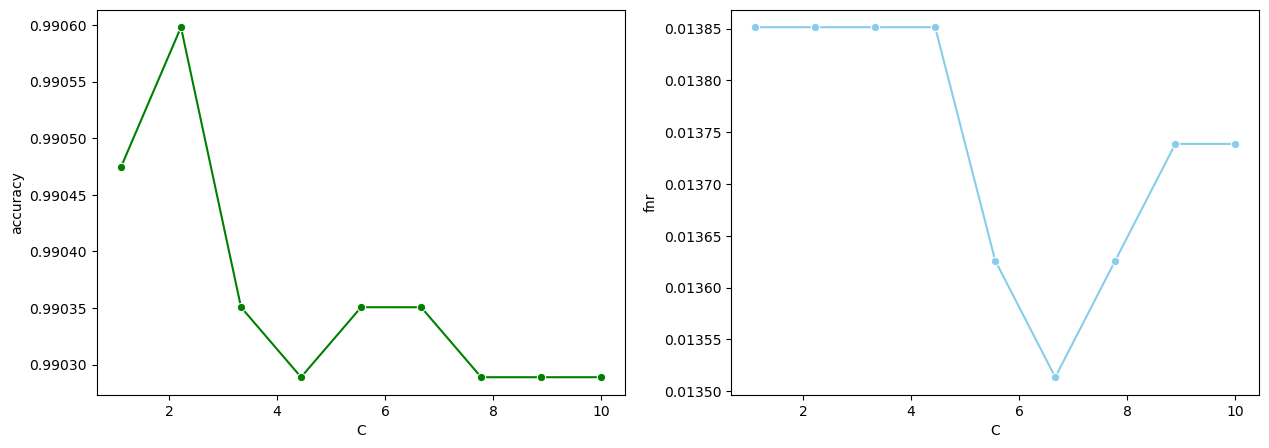
\includegraphics[width=1\linewidth]{linear_svm_accuracy_fnr.png}
	\caption{The plots show how the accuracy (left) and the FNR (right) change when the value of $C$ hyperparameter changes}
	\label{fig:linearsvm}
\end{figure}

% comments on linear SVM
The plot in figure \ref{fig:linearsvm} show that the variations in terms of Accuracy and FNR when different values of $C$ are used to train the linear SVM are not that evident. Here the results obtained with $C=10^{-6}$ where not reported because of the significatively worse results (88.67\% of accuracy and 2.94\% of FNR). \\
Summarizing the best results we obtained:
\begin{table}[ht!]
	\centering
	\begin{tabular}{|l|l|l|}
		\hline
		\textbf{C} & \textbf{Accuracy} & \textbf{FNR} \\ \hline
		2.22       & 99.06\%           & 1.38\%       \\ \hline
		6.67       & 99.03\%           & 1.35\%       \\ \hline
	\end{tabular}
\end{table}

Optimizing for the $FNR$ the hyperparameter we have selected is $C=6.67$.
\subsection{Kernel SVM}
% Why SVM are good: kernels
What it makes the SVMs particularly powerful is the way how the dual problem is defined. We are indeed able to embed a non-linear decision function that computes the scalar product between $x_i$ and $x_j$ in a higher dimensional space without needing to  explicitly compute the features expansion. A kernel function is defined as 
\begin{center}
	$k(x,y) = \Phi(x)^T\Phi(y)$
\end{center}
And the $J_D$ function is modified as:
\begin{center}
	$J_D(\alpha) = \sum_{i=1}^{n}\alpha_i -\frac{1}{2}\sum_{i=1}^{n}\sum_{j=1}^{n}\alpha_i\alpha_jz_iz_jk(x_i,x_j)$
\end{center}
Also the inference step is modified accordingly:
\begin{center}
	$y_t = w^Tx_t + w_0 = \sum_{i=1}^{n}\alpha_iz_ik(x_t,x_i)$
\end{center}
We have implemented a Radial Basis Function (RBF) kernel that is defined as:
\begin{center}
	$k(x,y) = e^{-\gamma||x-y||^2}$
\end{center}
% TODO: explain gamma hyperparameter
\subsubsection{Experiments}
% Results obtained with the RBF kernel SVM (plots)
The cross-validation of the model has now to take into account two different hyperparameters ($\gamma$ for the RBF kernel and $C$ for the dual SVM problem). 
This time we exploited a grid search k-fold cross validation that makes use of the cross validation to train the model with each possible combinations of hyperparameters. The hyperparameters values we tried are:
\begin{itemize}
	\item $\gamma$: 10 values in $[10^{-6}, 1]$
	\item $C$: 10 values in $[10^{-6}, 10]$
\end{itemize}
We now investigate the influence of both hyperparameters. What it's not displayed and analyzed in the plots is what happens with $C=10^{-6}$ and $\gamma=10^{-6}$, parameters under which the classifier performs a very poorly in terms of accuracy (around $54\%$) despite achieving a $FPR$ equal to $0\%$. However, this is not better than a dummy classifier that safely detects every PDF as malicious so it's not of interest in this project.

\begin{figure}[ht!]
	\centering
	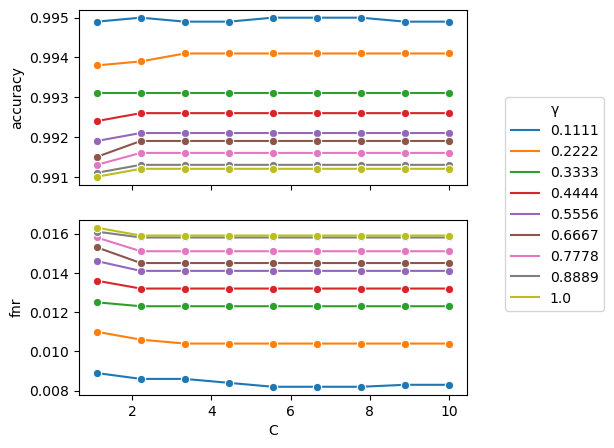
\includegraphics[width=1\linewidth]{rbf_svm_gamma_accuracy_fnr.png}
	\caption{Accuracy (top) and FNR (bottom) when $\gamma$ (colored lines) changes and $C$ changes}
	\label{fig:rbfsvmgamma}
\end{figure}

In figure \ref{fig:rbfsvmgamma} it's clear that smaller values of $\gamma$ lead to obtain better results both in terms of Accuracy and FNR. The $\gamma$ parameter of the RBF kernel controls the width of the kernel, it determines how far the influence of a single training example reaches, and how smooth the decision boundary is. A lower value of gamma means a larger, less concentrated kernel, which can lead to smoother decision boundaries.

We also investigated the role of the $C$ hyperparameter.

\begin{figure}[ht!]
	\centering
	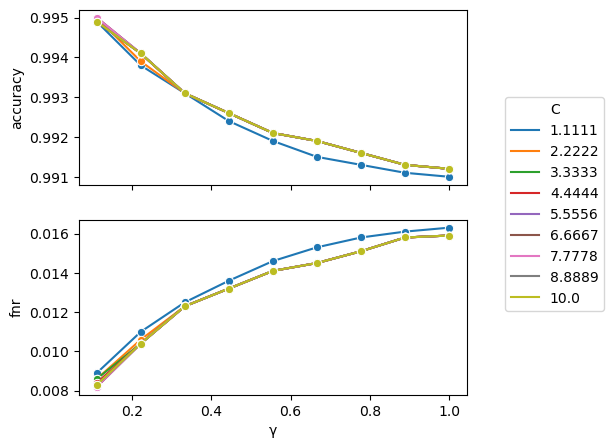
\includegraphics[width=1\linewidth]{rbf_svm_C_accuracy_fnr.png}
	\caption{Accuracy (top) and FNR (bottom) when $C$ (colored lines) changes and $\gamma$ changes}
	\label{fig:rbfsvmC}
\end{figure}

As we can observe in figure \ref{fig:rbfsvmC} the value of the $C$ hyperparameter has less influence on the model than $\gamma$. The $C$  hyperparameter controls the trade-off between the simplicity of the model (low bias, high variance) and the training error (low variance, high bias). A higher value of C means a higher penalty for misclassification while a lower value of C means a lower penalty for misclassification.\\
When the value of $\gamma$ is sufficiently small the accuracy reaches the best values and the same happens for the FNR. The choice of $C$ has clearly less impact on the performances. 

Overall the best values we have found from cross validation are:

\begin{table}[ht!]
	\centering
	\begin{tabular}{|l|l|l|l|}
	\hline
	\textbf{C} & \textbf{$\gamma$} & \textbf{Accuracy} & \textbf{FNR} \\ \hline
	5.56     & 0.11         & 99.50\%           & 0.82\%       \\ \hline
	\end{tabular}
\end{table}

\subsection{Performances on the test set}
Finally, given the set of best hyperparameters found through cross validation on the entire training set we are going to asses the performances achieved on the test set.
\subsubsection{Linear SVM}

\begin{table}[ht!]
	\centering
	\begin{tabular}{|l|l|l|}
		\hline
		\textbf{C} & \textbf{Accuracy} & \textbf{FNR} \\ \hline
		6.67       & 99.06\%           & 1.58\%       \\ \hline
	\end{tabular}
	\caption{Linear SVM - Performances on the test set}
\end{table}

\subsubsection{Kernel SVM}
Secondly we train a RBF SVM on the entire training set and we do the predictions on the entire testing set.
\begin{table}[ht!]
	\centering
	\begin{tabular}{|l|l|l|l|}
	\hline
	\textbf{C} & \textbf{$\gamma$} & \textbf{Accuracy} & \textbf{FNR} \\ \hline
	5.56     & 0.11         & 99.50\%           & 0.82\%       \\ \hline
	\end{tabular}
	\caption{RBF SVM - Performances on the test set}
\end{table}

%%# DECISION TREE AND RANDOM FOREST #%%
\section{Decision tree and random forest}
\label{sec:tree}
The decision tree is a popular classification technique in which predictions are made in a sequence of single-attribute tests.
A decision tree consists of three types of nodes:
\begin{itemize}
	\item decision nodes (squares)
	\item chance nodes (circles)
	\item end nodes (triangles)
\end{itemize}

Decision trees are used to evaluate the expected values or expected utility of competing alternatives. Each internal node in a decision tree represents a test on an attribute, and each branch represents the outcome of the test. The paths from the root to the leaf nodes represent classification rules, and the leaf nodes represent class labels.
In this test, we evaluated the performance of a decision tree using various parameters such as tree depth, minimum number of samples per leaf, and maximum number of features. We found that adjusting these parameters had a significant impact on the false negative rate and the accuracy of the model. For example, as shown in Figure 1, we found that the optimal tree depth parameter was 15, which provided the best balance between model performance and overfitting.
\subsection{Random forest}
Random Forest is a machine learning algorithm that is used for both classification and regression tasks. It is an ensemble method, which means that it combines the predictions of multiple decision tree models to make a more accurate and stable prediction.
To train a Random Forest model, multiple decision trees are trained on different samples of the data and their predictions are combined. This helps to reduce overfitting and improve the model's generalization ability. The algorithm is also robust to missing values, making it a versatile and widely used machine learning tool.
In our analysis we chose this model because of its high accuracy and stability. It is known for performing well on a wide range of datasets and tasks.
Also with Random Forest, we evaluated the performance varying parameters and in Figure we can see the results for maximum trees depth.

%%# KNN #%%
\section{KNN}
\label{sec:knn}
\paragraph{Algorithm}
\subsection{Experiments}

%%# FINAL RESULTS #%%
\section{Final results}
\label{sec:finalresults}

%%# ATTACKS TO CLASSIFIERS #%%
\section{Attacking the classifiers}
\label{sec:attacks}

%%# CONCLUSIONS #%%
\section{Conclusions and future works}
\label{sec:conclusions}

%%# CONTRIBUTIONS #%%
\section{Contributions}
\label{sec:contributions}

%%%%%%%%%%%% Supplementary Methods %%%%%%%%%%%%
%\footnotesize
%\section*{Methods}

%%%%%%%%%%%%% Acknowledgements %%%%%%%%%%%%%
%\footnotesize
%\section*{Acknowledgements}

%%%%%%%%%%%%%%   Bibliography   %%%%%%%%%%%%%%
\normalsize
\bibliography{references}

%%%%%%%%%%%%  Supplementary Figures  %%%%%%%%%%%%
%\clearpage

%%%%%%%%%%%%%%%%   End   %%%%%%%%%%%%%%%%
%\end{multicols}  % Method B for two-column formatting (doesn't play well with line numbers), comment out if using method A
\end{document}
